\documentclass[11pt,letterpaper]{article}
\usepackage{array}
\usepackage{fullpage}
\usepackage{graphicx}
\usepackage{parskip}
\usepackage{amsmath}
\usepackage[small]{caption}
\usepackage{graphpap}
\usepackage{logpap}
\usepackage{tabularx}
\usepackage{url}
\usepackage{hyperref}
\usepackage{enumitem}

\renewcommand{\thesection}{PART \arabic{section}: }

\newcounter{question}[section]
\newenvironment{question}[1][]{\refstepcounter{question}\par\medskip
   \textbf{\arabic{section}.\thequestion.} \rmfamily}{\medskip}

\usepackage{titlesec}
\titleformat{\section}{\clearpage\normalfont\bfseries}{\thesection}{0em}{}
\titlespacing{\section}{0pt}{0.5\baselineskip}{0pt}

\titleformat{\subsection}[runin]
{\normalfont\bfseries}{\thesubsection}{1em}{}

\titleformat{\subsubsection}{\normalfont\bfseries}{\thesubsubsection}{0em}{}
\titlespacing{\subsubsection}{0pt}{0.5\baselineskip}{0pt}

\newcounter{saveenumi}
\newcommand{\seti}{\setcounter{saveenumi}{\value{enumi}}}
\newcommand{\conti}{\setcounter{enumi}{\value{saveenumi}}}

\usepackage[dvipsnames]{xcolor}
\newcommand{\sol}[1]{{\color{NavyBlue} #1}}


\begin{document}
\setlength{\parindent}{0in}

%% EQUIP: Force Probe, Pulley, Track, Hangar, Weight, Tilt, Scale

\begin{flushright}
PHYS S123: College Physics I\\
Lab 5: Torque\\
10/7/25 (due 10/14/25)
\end{flushright}

Name(s):\\

\subsubsection*{Topics:}
\begin{enumerate}
\setlength{\parskip}{3pt}
\item Relationship between torque, moment of inertia, and rotational motion
\item Combination motion (rotational motion plus translational motion)
\end{enumerate}

\subsubsection*{Introduction:}
In this lab you will explore the concepts of rotational motion, rolling motion, and moment of inertia. In the first part of the lab, you will use a rotational motion apparatus to measure the moment of inertia for two objects. In the second part, you will compare the speed at which objects of different shapes, and therefore different moments of inertia, roll down an incline.  
 
Newton's second law, written for linear motion, has the familiar form $\sum \vec{F}=m\vec{a}$, and states that the linear acceleration that an object receives depends directly on the force acting on it
and inversely on its mass.  For the case of angular motion, we have seen that Newton's
second law takes the form $\sum\tau = I \alpha$. Here the angular acceleration depends directly on the torque acting on a body and inversely on its moment of inertia.  Moment of inertia is the
property of an object that describes its resistance to changes in angular velocity, just as mass is a measure of an object's resistance to changes in linear velocity. The moment of inertia depends on the mass of a body and how that mass is distributed --- its shape, size, and location of the rotational axis.

\subsubsection*{What you should turn in:} 
You may submit a group report.
\begin{enumerate}
\setlength{\parskip}{3pt}
\item Part 1: A free-body diagram [2 pts], the force balance equations and derivation you used to arrive at an equation for the moment of inertia [4 pts], and your measured and theoretical moments of inertia [4 pts].
\item Part 2: A derivation of the time it takes the object to roll down the ramp [4 pts], a table of the expected and observed travel times [2 pts], and a discussion of how ``rolling friction'' influences the motion of an object (i.e., discuss what sort of object's are most influenced by rolling friction) [2 pts].
\end{enumerate}

\subsubsection*{Equipment}
\begin{itemize}
\setlength{\parskip}{3pt}
\item Rotating apparatus and disks and rings
\item String and hanging masses
\item Scale
\item Rolling objects (disk and ring)
\item 2-m stick
\end{itemize}

\pagebreak
\subsubsection*{Additional background}
The moment of inertia can be calculated analytically for objects that have a lot of symmetry. In the table below, $m$ indicates the mass of the object, $d$ is the distance of the object from the axis of rotation, $R$ is the radius of the object, and $L$ is the length of a rod.

\renewcommand{\arraystretch}{2}
\begin{table}[h]
\begin{tabular}{|l|c|}
\hline
Object & Moment of inertia\\
\hline
Point mass & $md^2$\\
Cylinder & $\frac{1}{2}mR^2$\\
Thick-walled cylinder & $\frac{1}{2}m\left(R_{\rm inner}^2+R_{\rm outer}^2\right)$\\
Solid sphere & $\frac{2}{5}mR^2$\\
Spherical shell & $\frac{2}{3}mR^2$\\
Rod (around the center) & $\frac{1}{12}mL^2$\\
\hline
\end{tabular}
\end{table}

In part 1 of the lab, you will estimate and measure the moment of inertia of a disk, a ring, and a system of two point masses. The masses of the disks and rings are shown in the following table.
\begin{table}[h]
\begin{tabular}{|l|c|}
\hline
Object & Mass [kg]\\
\hline
Gray ring & 4.297\\
Gray disk & 4.825\\
Blue ring & 4.359\\
Blue disk & 4.975\\
Brown disk & 4.869\\
``Point'' masses & 2.703\\
Rod & 0.832\\
\hline
\end{tabular}
\end{table}

\section{MEASURING AN OBJECT'S MOMENT OF INERTIA}
For this part of the lab, a body is set in rotation about a vertical axis.  The applied
torque is from a constant force produced by a falling mass. Using force and torque balances, you will derive an expression in which the moment of inertia of the rotating body is related to measurable quantities. Additionally, since the moments of inertia of certain bodies may be calculated from their masses and physical dimensions (using the equations in the textbook, which are also reproduced in Part 2), the theoretical moments of inertia may be computed to check the measured values.

\begin{figure}[h]
\begin{center}
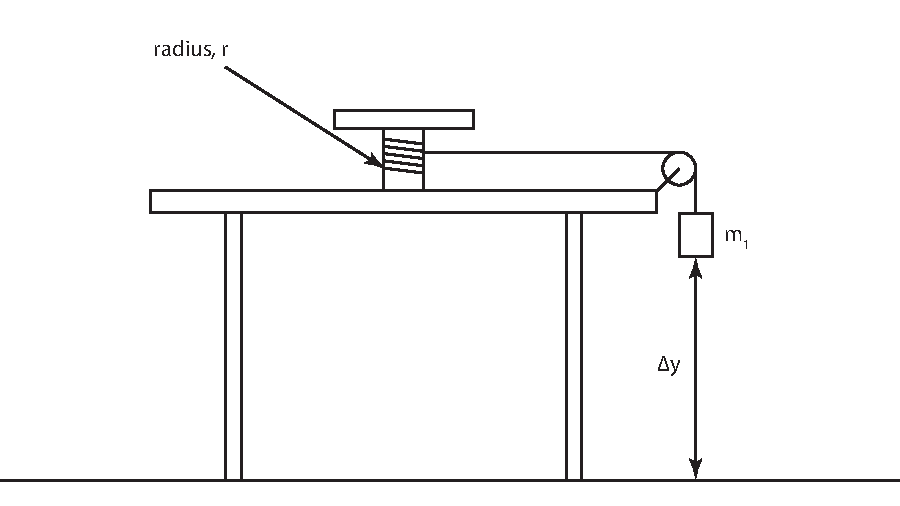
\includegraphics{./rotating_drum}
%\caption{Schematic of the lab experiment.}
\end{center}
\label{fig:schematic}
\end{figure}

This system is illustrated schematically in the figure above.  The body on the table is free to rotate about a vertical axis. This rotation occurs as the mass $m_1$ falls through a a distance $\Delta{y}$. The cord that constrains the motion of the mass $m_1$ is wound around the drum of the rotating body. The radius of the drum is $r$ and the rotating body has a moment of inertia $I_{\mbox{total}}$. The rotating body will consist of the apparatus plus a disk or ring that you place on top. Assume that the pulley is massless and frictionless.

Before performing any experiments, \textbf{draw a free body diagram} and use Newton's Second Law to \textbf{derive an expression for the moment of inertia of the rotating object} that depends on $m_1$, $r$, $\Delta y$, and $\Delta t$. Be sure that your derivation is correct before proceeding.

%The force balance on the hanging mass gives
%\begin{equation}
%\sum{F_y}=F_t-F_g=m_1a_y.
%\end{equation}
%Solving for the tensional force,
%\begin{equation}
%F_t=m_1(g+a_y).
%\label{eq:F_t}
%\end{equation}
%This tensional force is also the force that is causing the angular acceleration of the drum. The torque balance on the drum gives
%\begin{equation}
%\sum\tau=rF_t=I\alpha.
%\label{eq:sum_tau}
%\end{equation}
%The angular acceleration is related to the tangential acceleration by $a=\alpha{r}$, and therefore
%\begin{equation}
%I=\frac{r^2}{a}F_t
%\label{eq:I1}
%\end{equation}
%Inserting equation (\ref{eq:F_t}) into equation (\ref{eq:I1}) gives
%\begin{equation}
%I=\frac{m_1(g+a_y)r^2}{a}.
%\label{eq:I2}
%\end{equation}
%The tangential acceleration is given by the change in tangential speed $v>0$. Therefore an object whose rotation speeds up should have $a>0$. For this problem, the magnitude of the tangential acceleration is equal to the magnitude of the acceleration of the falling mass. Thus, $a=-a_y$ and
%\begin{equation}
%I=\frac{m_1(g+a_y)r^2}{-a_y}.5\label{eq:I3}
%\end{equation}
%Since the driving force is constant, mass $m_1$ will accelerate uniformly. The acceleration can be calculated by using the kinematic equations for constant acceleration (assuming no initial velocity):
%\begin{equation}
%\Delta{y}=\frac{1}{2}a\Delta{t}^2,
%\end{equation}
%and so
%\begin{equation}
%a=\frac{2\Delta{y}}{\Delta{t}^2}.
%\label{eq:a}
%\end{equation}
%Finally, inserting equation (\ref{eq:a}) into equation (\ref{eq:I3}) gives
%\begin{equation}
%I=\frac{m_1(g\Delta{t}+2\Delta{y})r^2}{-2\Delta{y}}.
%\end{equation}
%Therefore, the moment of inertia can be calculated by measuring the mass $m_1$, the radius of the drum $r$, and the time $\Delta{t}$ that it takes the mass to fall a distance $\Delta{y}<0$.

Now perform experiments in which you measure the variables needed to calculate the moment of inertia. %At least three measurements of each variable should be made, in order to allow averaging for better determination of the values.

{\bf Procedures:}\\  
1.  Measure the diameter of the drum around which
the cord is wound.\\
2.  Use a cord long enough so that the hanging weight can fall at least
1 meter.  Wind the cord around the drum.\\
3.  Make a practice run to make sure the apparatus is properly
set up.\\
%4.  Record the height at which you release the mass.  Use a stop watch
%to record the time it takes to fall that distance.\\

The rotating apparatus has a moment of inertia even without the ring or disk. You will need to take this into account when calculating the moment of inertia of the ring/disk. Because the apparatus and the ring/disk have the same axis of rotation, we can write
$$I_{\mbox{total}}=I_{\mbox{ring}}+I_{\mbox{apparatus}}$$
When you perform the experiments you will be calculating $I_{\mbox{total}}$. To calculate $I_{\mbox{ring}}$, you will therefore need to also know $I_{\mbox{apparatus}}$, which you can determine by running the experiment without the ring/disk. You will perform this experiment for two objects --- a disk and a ring.  Measure the physical mass and dimensions of the objects.\bigskip

{\bf Free body diagram and force balance derivation}\\
Sketch a free body diagram and use Newton's Laws to derive an expression for the moment of inertia of rotating apparatus.

\clearpage
{\bf Measured and theoretical moments of inertia}\\
Use the experimental values and the equation that you derived to calculate
the moment of inertia of the ring and the disk.


\renewcommand{\arraystretch}{1.4}
\begin{table}[h!]
\begin{tabular}{|c|c|c|c|c|c|c|c|}
\hline
& $m_1$ [kg] & $r$ [m] & $\Delta y$ [m] & $\Delta t$ [s] & $I_{total}$ [kg$\cdot$m$^2$] & $I_{object}$ [kg$\cdot$m$^2$]\\
\hline Platform & \hspace{1.5cm} & \hspace{1.5cm} & \hspace{1.5cm} & \hspace{1.5cm} & \hspace{1.5cm} & N/A\\
\hline Disk & & & & & & \\
\hline Ring & & & & & & \\
\hline Rod & & & & & &\\
\hline 2 point masses & & & & & &\\
\hline
\end{tabular}
\end{table}

Next, calculate the theoretical moments of inertia using the formulas on page 2 of the handout.

\begin{table}[h!]
\begin{tabular}{|c|c|c|c|c|c|c|c|}
\hline
& $I_{theoretical}$ [kg$\cdot$m$^2$]\\
\hline Disk & \hspace{1.5cm}\\
\hline Ring & \\
\hline Rod & \\
\hline 2 point masses & \\
\hline
\end{tabular}
\end{table}

How do your measured and theoretical values compare?



%\vspace{1cm}
%
%\newcolumntype{Y}{>{\centering\arraybackslash}X}%
%\begin{tabularx}{\linewidth}{|Y|Y|Y|Y|Y|}
%\hline
%no disk or ring & $m_1$ & $r$ & $\Delta{t}$ & $\Delta{y}$ \\
%\hline\vspace{2cm}&\vspace{2cm}&\vspace{2cm}&\vspace{2cm}&\vspace{2cm}\\
%\hline\vspace{2cm}&\vspace{2cm}&\vspace{2cm}&\vspace{2cm}&\vspace{2cm}\\
%\hline\vspace{2cm}&\vspace{2cm}&\vspace{2cm}&\vspace{2cm}&\vspace{2cm}\\
%\hline\vspace{2cm}&\vspace{2cm}&\vspace{2cm}&\vspace{2cm}&\vspace{2cm}\\
%\hline\hline AVERAGE:&\vspace{2cm}&\vspace{2cm}&\vspace{2cm}&\vspace{2cm}\\
%\hline
%\end{tabularx}\\
%
%\vspace{1cm}
%
%\newcolumntype{Y}{>{\centering\arraybackslash}X}%
%\begin{tabularx}{\linewidth}{|Y|Y|Y|Y|Y|}
%\hline
%ring & $m_1$ & $r$ & $\Delta{t}$ & $\Delta{y}$ \\
%\hline\vspace{2cm}&\vspace{2cm}&\vspace{2cm}&\vspace{2cm}&\vspace{2cm}\\
%\hline\vspace{2cm}&\vspace{2cm}&\vspace{2cm}&\vspace{2cm}&\vspace{2cm}\\
%\hline\vspace{2cm}&\vspace{2cm}&\vspace{2cm}&\vspace{2cm}&\vspace{2cm}\\
%\hline\vspace{2cm}&\vspace{2cm}&\vspace{2cm}&\vspace{2cm}&\vspace{2cm}\\
%\hline\hline AVERAGE:&\vspace{2cm}&\vspace{2cm}&\vspace{2cm}&\vspace{2cm}\\
%\hline
%\end{tabularx}\\
%
%\vspace{1cm}
%
%
%%\newcolumntype{Y}{>{\centering\arraybackslash}X}%
%\begin{tabularx}{\linewidth}{|Y|Y|Y|Y|Y|}
%\hline
%disk & $m_1$ & $r$ & $\Delta{t}$ & $\Delta{y}$ \\
%\hline\vspace{2cm}&\vspace{2cm}&\vspace{2cm}&\vspace{2cm}&\vspace{2cm}\\
%\hline\vspace{2cm}&\vspace{2cm}&\vspace{2cm}&\vspace{2cm}&\vspace{2cm}\\
%\hline\vspace{2cm}&\vspace{2cm}&\vspace{2cm}&\vspace{2cm}&\vspace{2cm}\\
%\hline\vspace{2cm}&\vspace{2cm}&\vspace{2cm}&\vspace{2cm}&\vspace{2cm}\\
%\hline\hline AVERAGE:&\vspace{2cm}&\vspace{2cm}&\vspace{2cm}&\vspace{2cm}\\
%\hline
%\end{tabularx}\\





\section{MOTION OF AN OBJECT ROLLING DOWN A SLOPE}
For this part of the lab, you will compare the motion of two solid cylinders and two hollow cylinders as they roll down an inclined plane. For each object, measure the mass and radius so that you can compare the measured travel times with theoretically expected travel times. 



\begin{figure}[h]
\begin{center}
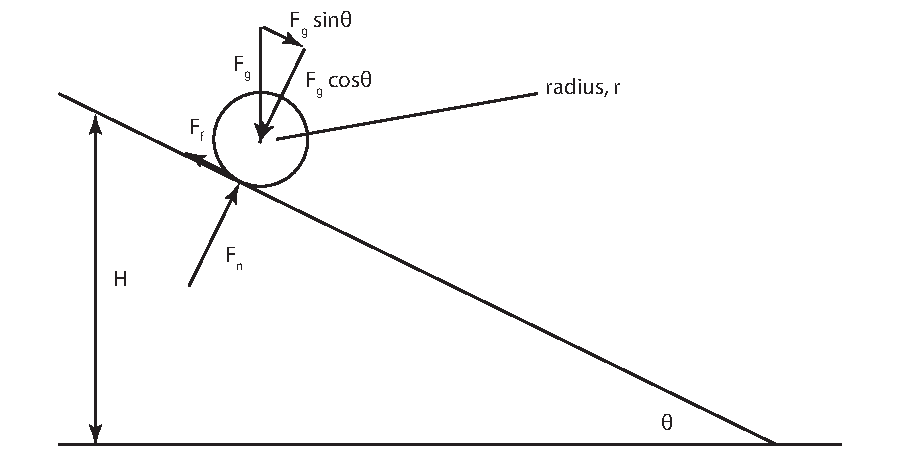
\includegraphics{./rolling_ball}
\end{center}
\end{figure}



%The velocity of a rolling object's center of mass can be found by computing the force and torque balances on the object, so that
%\begin{equation}
%\sum{F_x}=F_g\sin\theta-F_f=ma
%\label{eq:F_x}
%\end{equation}
%and
%\begin{equation}
%\sum{\tau}=-F_f r = I\alpha = -I\frac{a}{r}.
%\label{eq:tau}
%\end{equation}
%The torque is negative for clockwise rotation. In this case, $\alpha=-a/r$ because $a$ is defined to be positive in the clockwise direction. Solving equation (\ref{eq:tau}) for $F_f$ and inserting the result into equation (\ref{eq:F_x}) gives
%\begin{equation}
%F_g\sin\theta-I\frac{a}{r^2}=ma.
%\end{equation}
%Solving for $a$ yields
%\begin{equation}
%a=\frac{mr^2g\sin\theta}{I+mr^2}.
%\label{eq:a}
%\end{equation}
%Equation (\ref{eq:a}) indicates how quickly an object rolling down a ramp will accelerate. We can now use the kinematic equations to determine how long it will take an object to roll down a ramp. If the object is released from a height of $H$, then it will travel a distance of 
%\begin{equation}
%\Delta{x}=\frac{H}{\sin\theta}=\frac{1}{2}a\Delta{t}^2.
%\label{eq:Delta_x}
%\end{equation}
%The time that it takes the object to roll that distance, from a state of rest, is 
%\begin{equation}
%\Delta{t}=\displaystyle\sqrt\frac{2H}{a\sin\theta}=\displaystyle\sqrt\frac{2H(I+mr^2)}{mr^2g\sin^2\theta}.
%\label{eq:Delta_t1}
%\end{equation}
%\textit{If} the moment of inertia were not accounted for, then equation (\ref{eq:Delta_t1}) would reduce to
%\begin{equation}
%\Delta{t}=\displaystyle\sqrt\frac{2H}{g\sin^2\theta},
%\label{eq:Delta_t2}
%\end{equation} 
%which is exactly the same solution you would get if you analyzed a box sliding down a frictionless ramp.


%to solve for the object's velocity at the bottom of the ramp. 
%\begin{equation}
%\left(v_f\right)^2-\left(v_i\right)^2=2a\Delta{x}
%\label{eq:v_f^2}
%\end{equation}
%The initial velocity is $v_i=0$, and $\Delta{x}=H/\sin\theta$. Inserting these relationships and equation (\ref{eq:a}) into equation (\ref{eq:v_f^2}), we find that
%\begin{equation}
%v_f=\sqrt{\frac{mr^2gH}{I+mr^2}}.
%\label{eq:v_f}
%\end{equation}
%Note that if $I\ll{mr^2}$, then 
%\begin{equation}
%v_f\approx\sqrt{gH}.
%\end{equation}
%This approximation was used in the momentum lab. 
First, derive an expression for the time that it takes the object to roll down the ramp. Assume that the objects roll without slipping. The result will depend on the object's moment of inertia, which can be computed using the equations on page 2 of the handout.

{\bf Derivation of the time that it takes the object to roll down the ramp}

\clearpage

Record the shape, mass, and radii of each of the four objects. For the hollow cylinders, you will need both the inner and outer radii.

\begin{table}[h!]
\begin{tabular}{|c|c|c|c|c|c|c|c|}
\hline
& $m$ [kg] & $r_{\rm outer}$ [m] & $r_{\rm inner}$ [m] & $I$ [kg$\cdot$m$^2$] & Expected $\Delta{t}$ [s] & Expected $\Delta{t}$ [s]\\
& & & & & (including friction) & (ignoring friction)\\
\hline Object 1 & \hspace{1.5cm} & \hspace{1.5cm} & \hspace{1.5cm} & \hspace{1.5cm} & \hspace{1.5cm} & \hspace{1.5cm} \\
\hline Object 2 & & & & & & \\
\hline Object 3 & & & & & & \\
\hline Object 4 & & & & & & \\
\hline
\end{tabular}
\end{table}

Record the amount of time it actually takes the objects to roll down the ramp. Do three trials for each object and calculate the average $\Delta{t}$.
\begin{table}[h!]
\begin{tabular}{|c|c|c|c|c|}
\hline & $\Delta{t_1}$ [s] & $\Delta{t_2}$  [s] & $\Delta{t_3}$ [s] & $\Delta{t_4}$  [s] \\
\hline Trial 1 & \hspace{3cm} &\hspace{3cm} & \hspace{3cm} & \hspace{3cm} \\
\hline Trial 2 & & & & \\
\hline Trial 3 & & & & \\
\hline\hline AVERAGE: & & & & \\
\hline
\end{tabular}
\end{table}


{\bf How does ``rolling motion'' influence the motion of an object? In other words, compare your results to what would happend with a frictionless surface, and discuss how the mass distribution affects your results. }

Compare these results to the expected values of $\Delta{t}$. For which objects did the rotational motion have the biggest effect on travel time? How much did including rolling friction change your results?

Note that you need to describe your observations both qualitatively and quantitatively. To help with interpreting the results (and as a check that your measurements and calculations are consistent), it may be helpful to do a series of head-to-head races with the different shapes. Which object accelerated most quickly? Least quickly?





\clearpage
\null


\end{document}
